\documentclass[a4paper,12pt]{report}
\usepackage[T2A]{fontenc}
\usepackage[utf8]{inputenc}
\usepackage[english,russian]{babel}
\usepackage{graphicx}
\usepackage{wrapfig}
\usepackage{mathtext} 				% русские буквы в фомулах
\usepackage{amsmath,amsfonts,amssymb,amsthm,mathtools} % AMS
\usepackage{icomma} % "Умная" запятая: $0,2$ --- число, $0, 2$ --- перечисление
\usepackage{capt-of}
\usepackage{appendix}
\usepackage{multirow}
\usepackage{hyperref}
\usepackage{floatrow}
\usepackage[left=2cm,right=2cm,
    top=2cm,bottom=2cm,bindingoffset=0cm]{geometry}
\usepackage{multicol} % Несколько колонок
\usepackage{gensymb}
\title{Отчёт по лабораторной работе №18

Вибрационный магнитометр}
\author{Богатова Екатерина}
\date{\today}

\begin{document}

\maketitle


\section*{1. Теоретические данные}

Метод заключается в следующем: образец намагничивается постоянным магнитным полем зазоре электромагнита и одновременно приводится периодическое движение с низкой частотой. Поля рассеяния, обусловленные намагниченностью вибрирующего образца, создают осциллирующий магнитный поток в расположенной поблизости измерительной катушке. Согласно явлению электромагнитной индукции в катушке возникает переменное напряжение (ЭДС индукции), которое и является мерой намагниченности вещества (сравнивается с ЭДС от эталонного образца). 

Математически принцип электромагнитной индукции описывается на основе закона Био-Савара:
\[ \varepsilon = -\cfrac{d\Phi}{dt}\]

Здесь $\varepsilon$ - ЭДС индукции, $\Phi$ - магнитный поток. При этом $\Phi = BSn$, $B$ - индукция, $S$ - площадь витка, $n$ - количество витков. Для небольших по амплитуде колебаний штока имеет место следующее соотношение: $\Delta B \propto A sin( \omega t)$, где $\Delta B$ - разность в величине индукции по площади витка при крайних положениях штока, $А$ - амплитуда колебаний штока, $\omega$ - частота колебаний. Тогда $\varepsilon \propto -n S \omega A cos( \omega t)$

В нашей установке колебания происходят параллельно магнитному полю, а ось измерительных катушек (в количестве 2 штук) направлена перпендикулярно. Важнейшим параметром магнитометров является чувствительность, т.е. минимальная величина магнитного момента, которую они могут устойчиво и воспроизводимо измерять.

Установлено, что чувствительность зависит как от конструкционных особенностей,
так и от экспериментальных условий. В связи с этим рассчитать оптимальную конструкцию с целью достижения заданной величины чувствительности весьма затруднительно.

\section*{2. Экспериментальная установка}
\begin{figure}[H]
    \centering
    \includegraphics[width=0.6\linewidth]{setup.png}
    \caption{Блок-схема вибромагнитометра.} \label{ustanovka}
\end{figure}

Блок-схема вибромагнитометра представлена на рисунке \ref{ustanovka}. Принцип работы заключается в следующем: вибропреобразователь (1), питаемый от генератора синусоидального тока (6), приводит в поступательное периодическое движение шток (2) с образцом (3). Образец находится под воздействием постоянного намагничивающего поля от электромагнита (5). В результате в приемных катушках (4) наводится ЭДС индукции. Образовавшееся напряжение поступает на вход селективного усилителя (8), а с выхода усиленный сигнал поступает сигнал с генератора (6). В результате на выходе детектора (7) образуется постоянный по амплитуде сигнал, пропорциональный амплитуде ЭДС индукции, а следовательно, и величине магнитного момента образца (3). Таким образом осуществляется на практике принцип синхронного детектирования.

\section*{3. Результаты эксперимента и обработка данных}

Чтобы найти оптимальный режим работы установки, подадим на катушку постоянный ток $I = $ А и будем менять частоту переменного сигнала, при этом фиксируя показания синхронного детектора. Так как показания синхронного детектора пропорциональны амплитуде полезного сигнала, при максимальных показаниях синхронного детектора амплитуда полезного сигнала будет максимальной. Полученная зависимость показана на рисунке \ref{afc}. Из графика получаем, что оптимальная частота колебаний $ f_{опт} = 35$ Гц.

\begin{figure}[H]
    \centering
    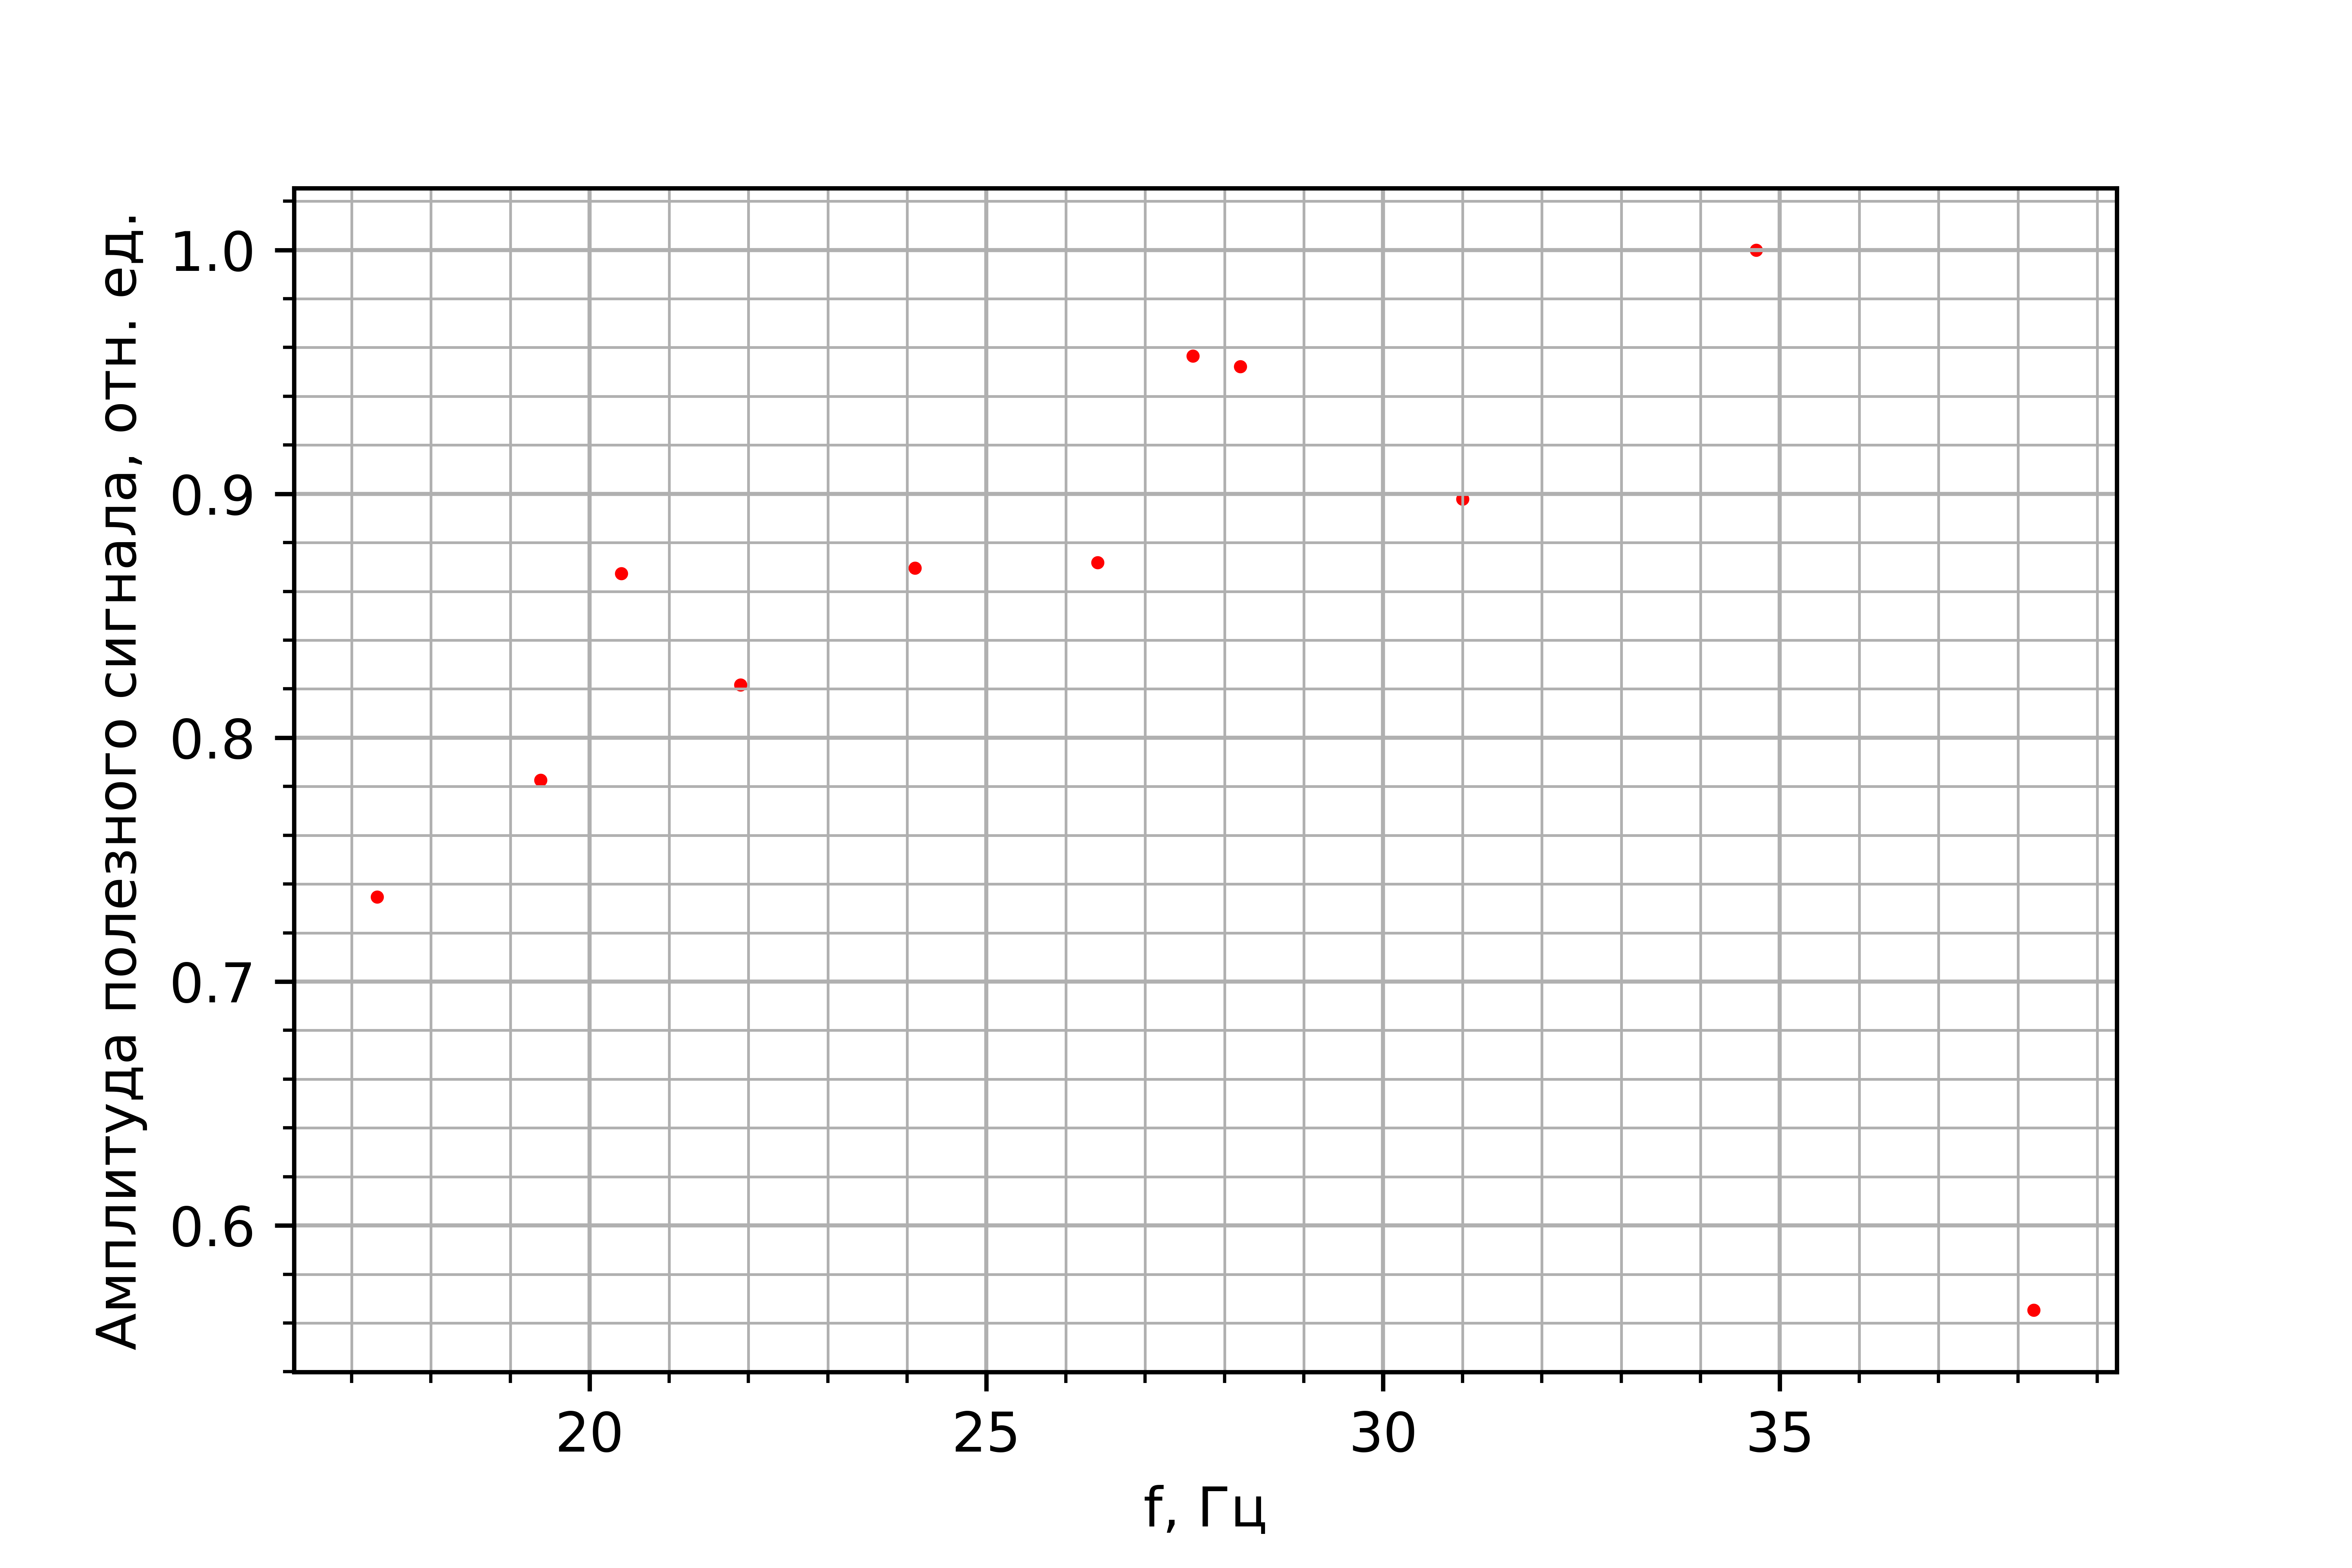
\includegraphics[width=0.6\linewidth]{Am(f)_Kate.png}
    \caption{Зависимость амплитуды полезного сигнала от частоты колебаний установки.} \label{afc}
\end{figure}

Найдем зависимость намагниченности образца от величины магнитного поля, создаваемого катушкой. Для этого выставим на генераторе найденную оптимальную частоту колебания и снимем зависимость показаний синхронного детектора от величины постоянного тока в катушке. Полученная зависимость показана на рисунке \ref{mu}

\begin{figure}[H]
    \centering
    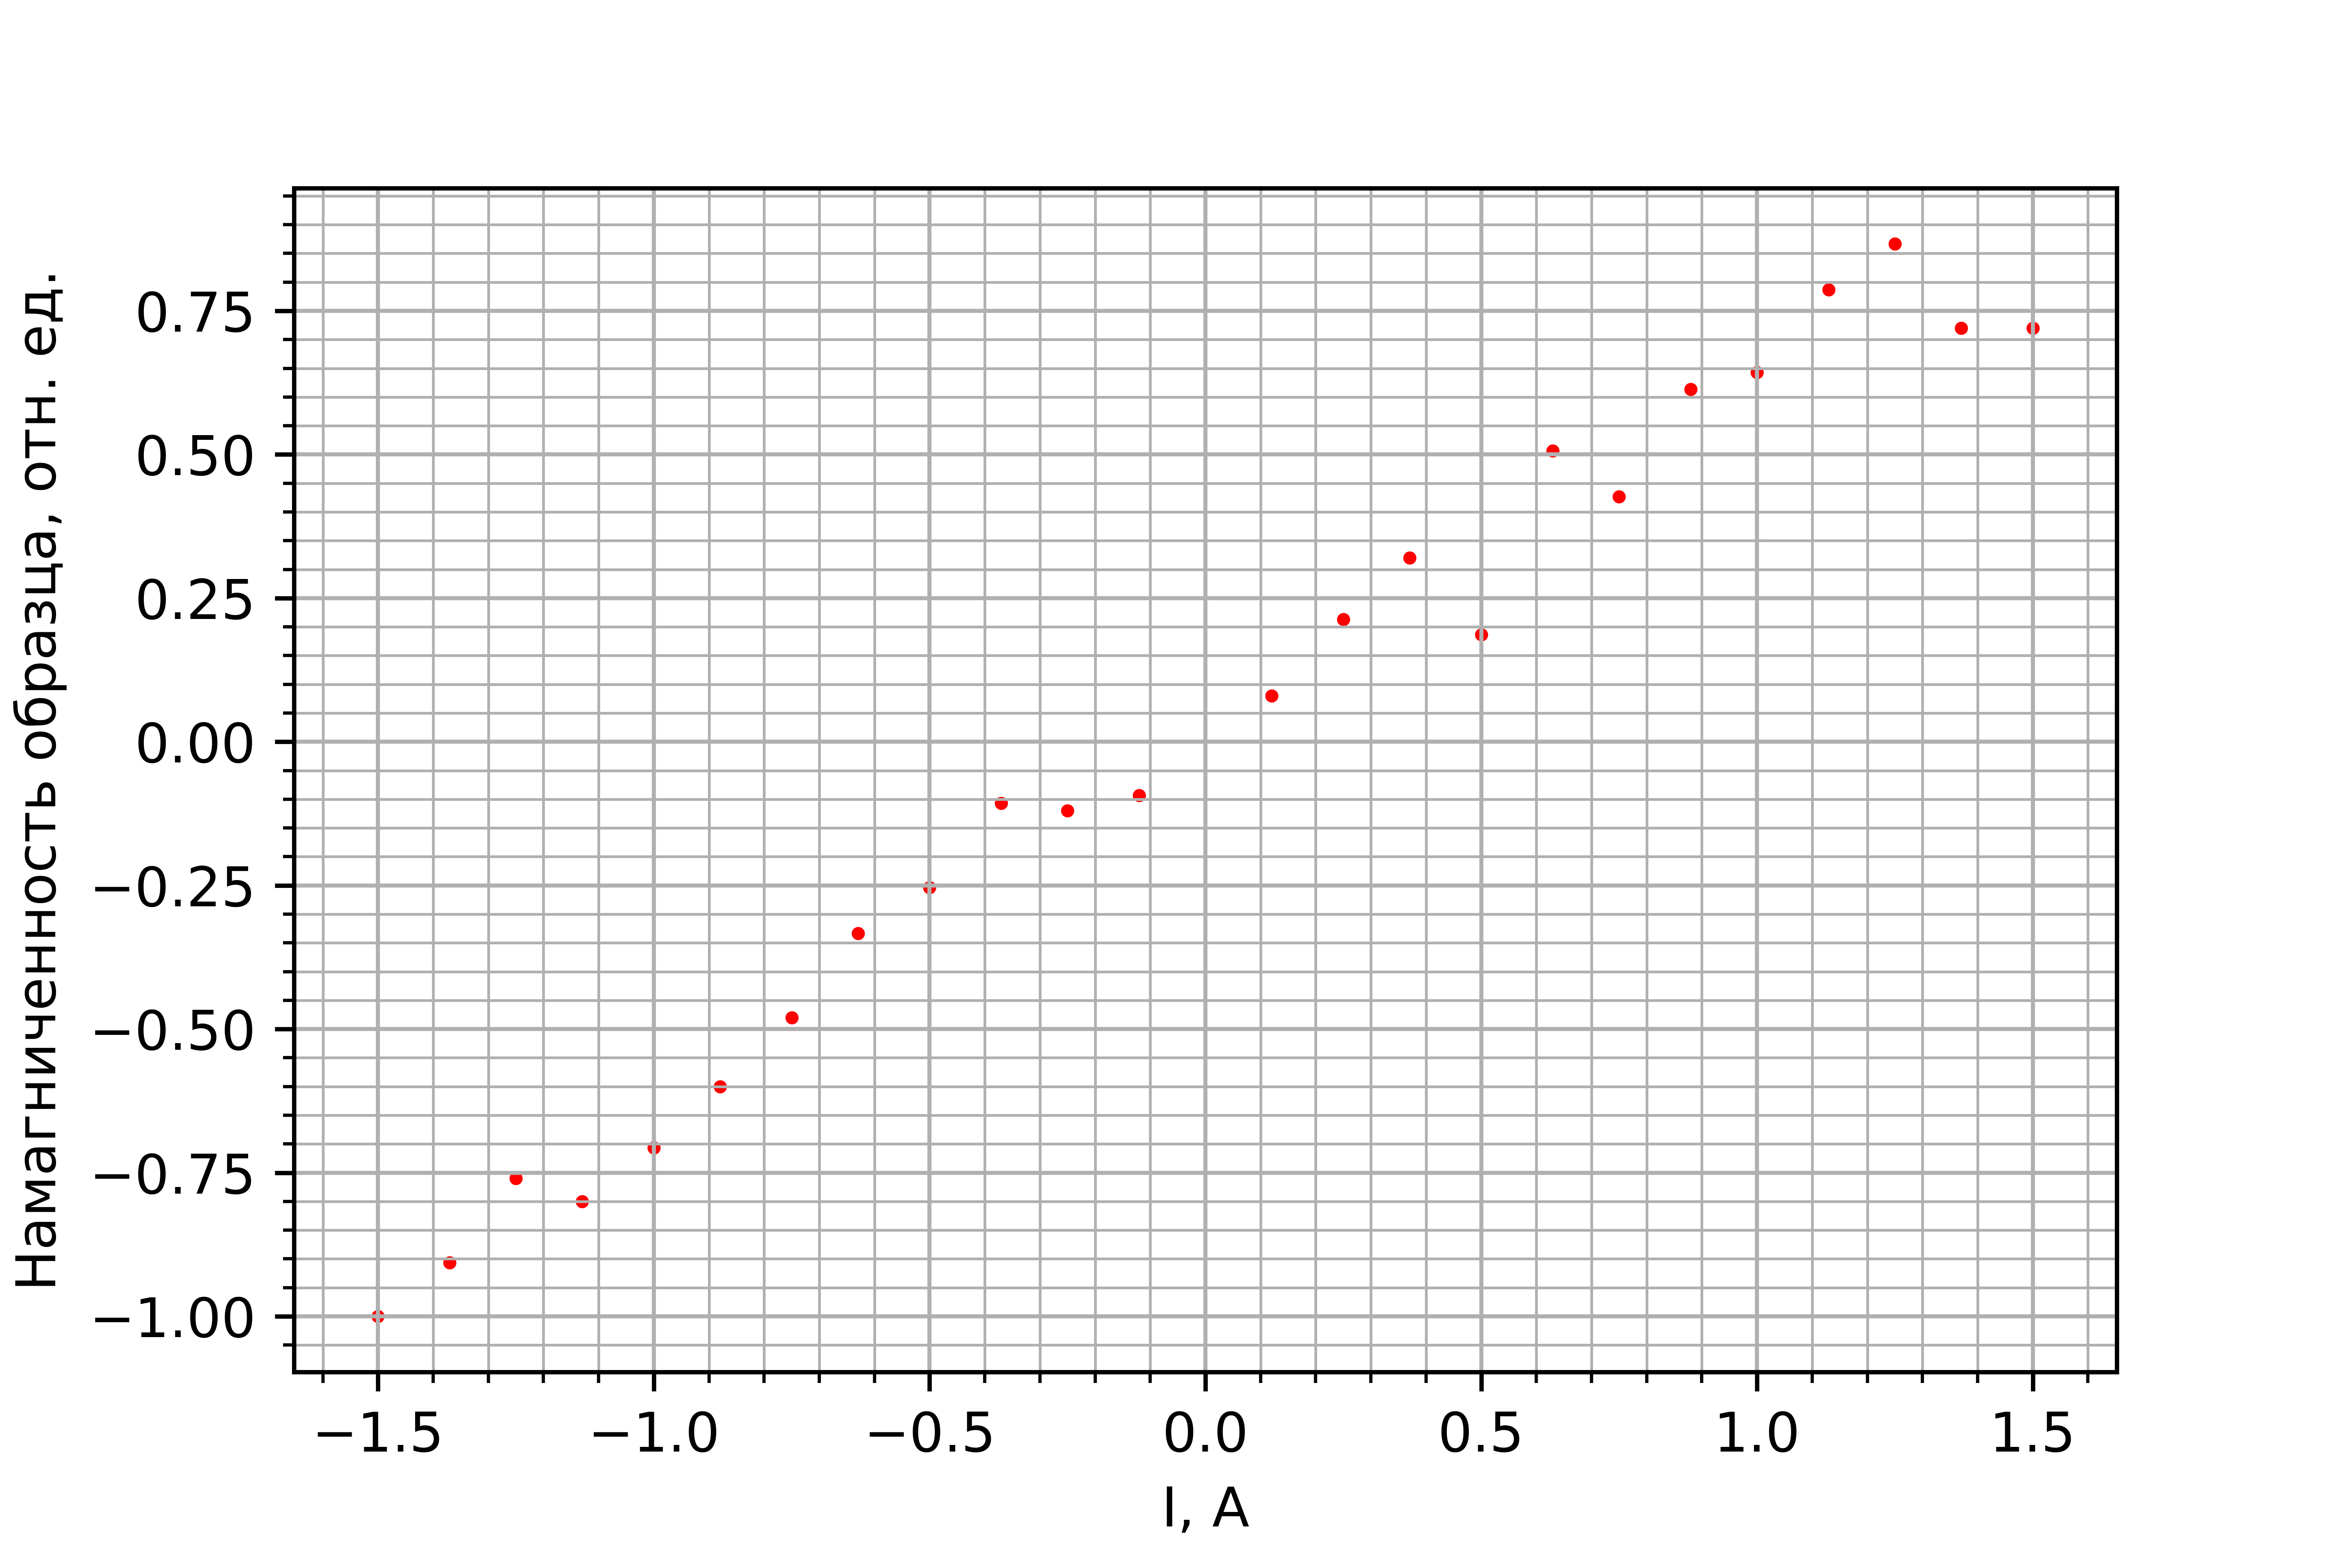
\includegraphics[width=0.6\linewidth]{Am(I)_Kate.png}
    \caption{Зависимость намагниченности образца от напряженности постоянного магнитного поля.} \label{mu}
\end{figure}

\section*{4. Вывод}

В данной работе были изучены основы конструирования и применения магнитометров с вибрирующим образцом для определения магнитных параметров тонкой магнитной пленки. В процессе работы мы получили зависимость амплитуды полезного сигнала от частоты колебаний установки, а также зависимость намагниченности образца от напряженности постоянного магнитного поля.


\end{document}
